\documentclass{article}
\usepackage[margin=1.5cm]{geometry}
\usepackage{amsmath}
\usepackage{graphicx}
\usepackage{booktabs}
\usepackage[utf8]{inputenc}
\usepackage{ragged2e}
\usepackage{paracol}
\setlength{\emergencystretch}{3em}
\begin{document}
\sloppy

\noindent\hfill
\includegraphics[height=1.8em]{assets/figure_header_logo.png}\par\noindent\hrule\vspace{4pt}
\begin{paracol}{2}
\RaggedRight

Health Monit. 2025;10(3):e13412. doi: 10.25646/13412


unterschied der bei Frauen bis zu 1,8 Prozentpunkte (Altersgruppe 7579 Jahre) niedriger liegt (Abbildung 1 und Annex Tabelle1).


Die beobachtete regionale Verteilung der 10-Jahres- Schlaganfallprävalenz zeigt kleinräumige Unterschiede mit einem Nordost-Süd-Gefälle (Abbildung 2, Annex Tabelle 2).

\switchcolumn
\RaggedRight

Nach Altersstandardisierung flachen diese Unterschiede deutlich ab. Die niedrigsten altersstandardisierten Prävalenzen (1,01,1\%) finden sich für das Jahr 2022 vor allem in süddeutschen (bzw. teils südwestdeutschen) Regionen wie Hochrhein-Bodensee sowie in einigen Metropolregionen (z. B. München, Rhein-Main, Stuttgart). Die höchsten Prä-

\end{paracol}


\begin{center}
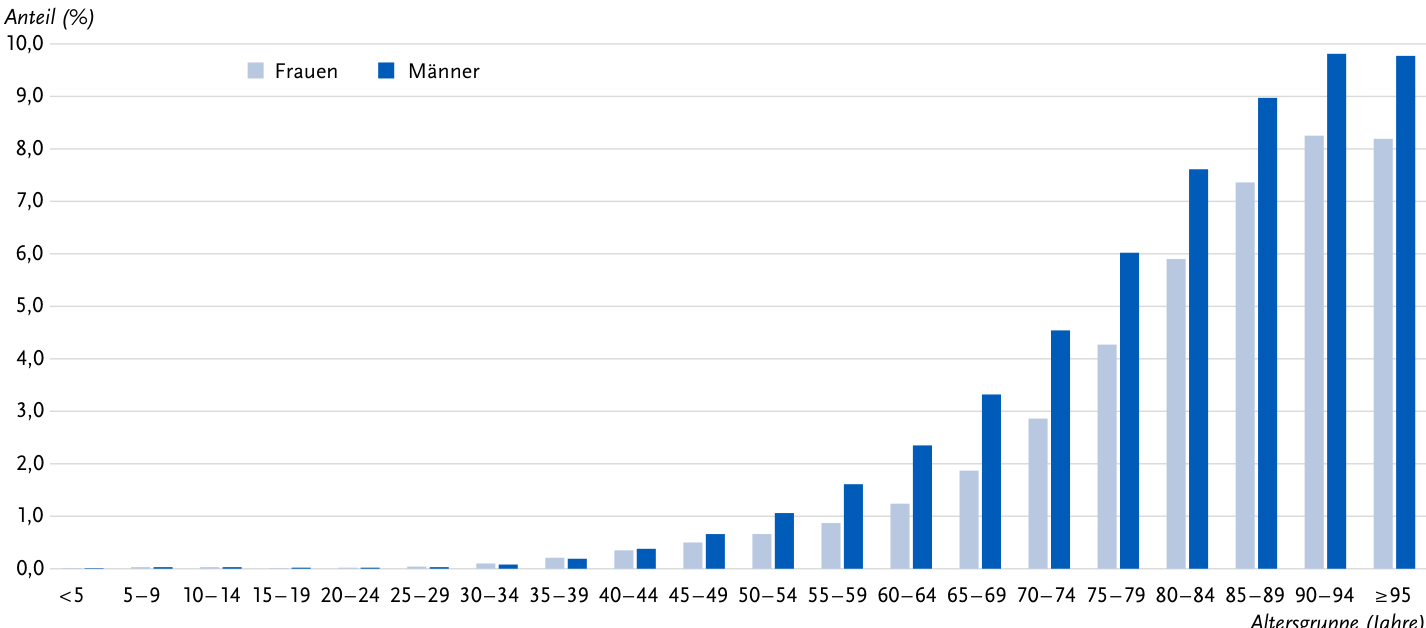
\includegraphics[width=0.8\linewidth]{assets/figures/figure_001.png}
\end{center}


Abbildung 1: 10-Jahres-Prävalenz von Schlaganfall nach Alter und Geschlecht (Bevölkerungsanteil in \%). Quelle: Krankheitslaststudie für Deutschland (AOK-Routinedaten 2022, alters-, geschlechtsund morbiditätsadjustiert und hochgerechnet auf die Bevölkerung Deutschlands)


\begin{center}
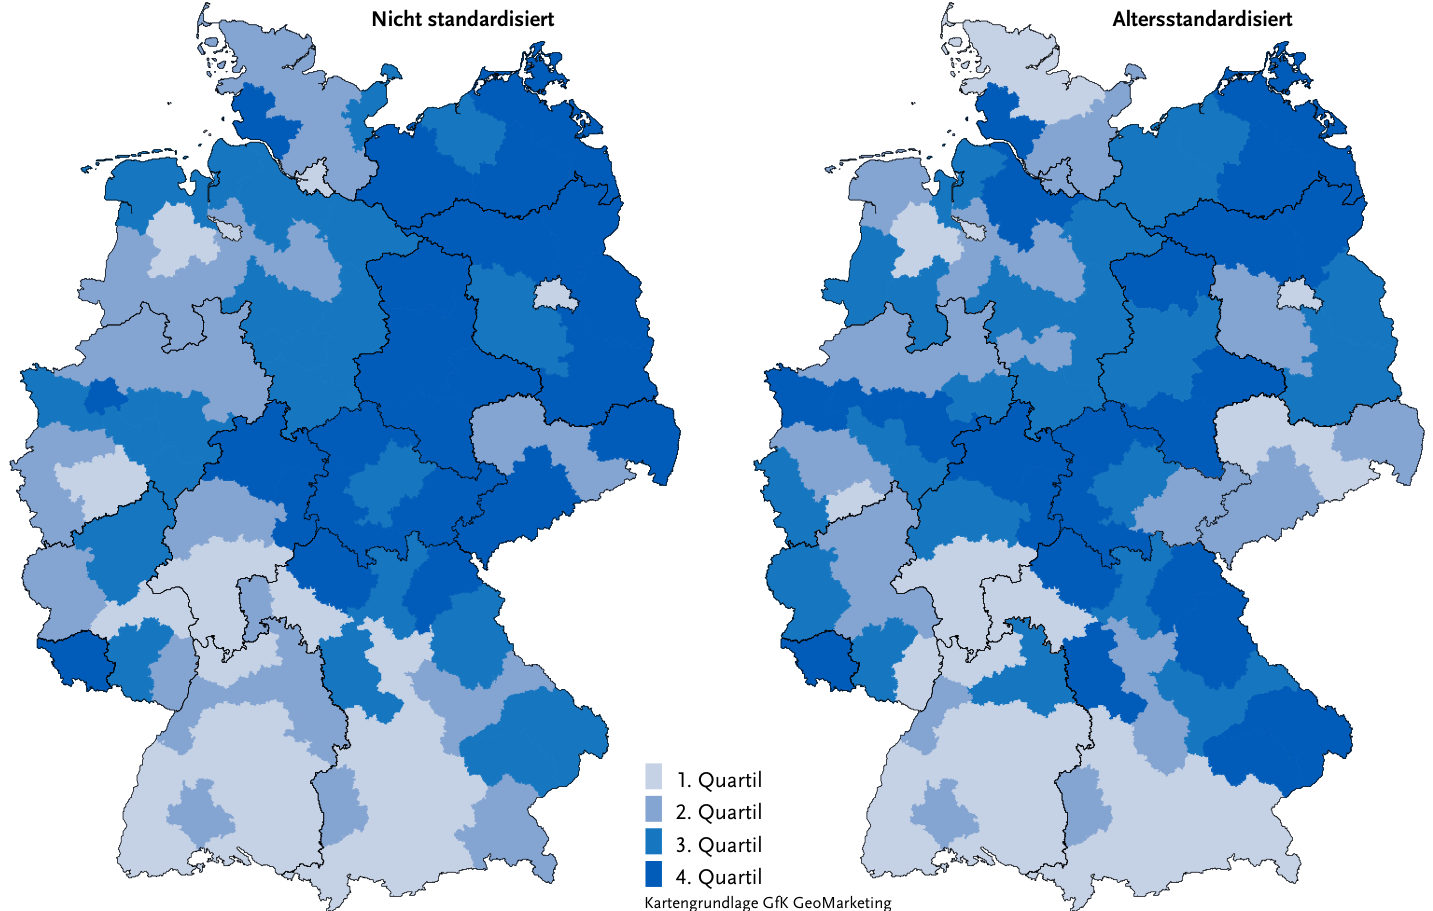
\includegraphics[width=0.8\linewidth]{assets/figures/figure_002.png}
\end{center}


\textit{Abbildung 2: 10-Jahres-Prävalenz von Schlaganfall nach Raumordnungsregionen (Anteil an der Bevölkerung in \%, Klasseneinteilung nach Quartilen). Quelle: Krankheitslaststudie für Deutschland (AOK-Routinedaten 2022, alters-, geschlechtsund morbiditätsadjustiert und hochgerechnet auf die Bevölkerung Deutschlands)}

\end{document}
